\documentclass{beamer}
\usepackage[utf8]{inputenc}
\usepackage[english]{babel}

% -- Including some standard packages --
\usepackage{graphicx}
\usepackage{soul}
\usepackage{hyperref}
\usepackage{colortbl}
\usepackage{dsfont}
\usepackage{soul}

% -- Choosing theme --

\usetheme{Boadilla}
\usecolortheme{whale}
\setbeamercolor{alerted text}{fg=purple} % Making alerted text non-red

% Tikz
\usepackage{tikz}
\usetikzlibrary{matrix,positioning,fit,backgrounds,intersections}

% Code highlighting
\usepackage{listings,lstautogobble}

% -- Cross signs --
\usepackage{pifont} % http://ctan.org/pkg/pifont
\newcommand{\cmark}{\ding{51}}%
\newcommand{\xmark}{\ding{55}}%
\newcommand{\xopt}{\ding{48}}%

\usepackage{listings}

% -- Custom commands --
\DeclareMathOperator*{\argmax}{arg\,max}
\DeclareMathOperator*{\argmin}{arg\,min}

\title[zk-SNARK I]{\textbf{zk-SNARK}}
\author{Distributed Lab}
\date{Sep 5, 2024}
\titlegraphic{
    
\includegraphics[width=\textwidth]{images/banner_wide.png}
}

\expandafter\def\expandafter\insertshorttitle\expandafter{%
  \insertshorttitle\hfill%
  \insertframenumber\,/\,\inserttotalframenumber}

\AtBeginSection[]{
  \begin{frame}
  \vfill
  \centering
  \begin{beamercolorbox}[sep=8pt,center,shadow=true,rounded=true]{title}
    \usebeamerfont{title}\insertsectionhead\par%
  \end{beamercolorbox}
  \vfill
  \end{frame}
}

\begin{document}
    \frame {
        \titlepage
    }

    \begin{frame}{Plan}
        \tableofcontents
    \end{frame}

    \section{What is zk-SNARK?}

    \begin{frame}{What Is zk-SNARK?}
        \begin{definition}
            \textbf{zk-SNARK} – Zero-Knowledge Succinct Non-interactive ARgument of 
            Knowledge.
        \end{definition}

        \pause

        \begin{itemize}
            \item \textbf{Argument of Knowledge} --- a proof that the prover knows the data (witness) that resolves a certain
            problem, and this knowledge can be ``extracted''. \pause
            \item \textbf{Succinctness} --- the proof size and verification time is relatively small relative to the computation size and typically does not depend on the size of 
            the data or statement. \pause
            \item \textbf{Non-interactiveness} --- to produce the proof, the prover does not need any interaction
            with the verifier. \pause
            \item \textbf{Zero-Knowledge} --- the verifier learns nothing about the data used to produce the
            proof, despite knowing that this data resolves the given problem and that the prover possesses it.
        \end{itemize}
    \end{frame}

    \begin{frame}{Still didn't get who is Snark...}
        Well... Let's take a look at some example. \pause

        \begin{columns}
            \begin{column}{0.2\textwidth}
                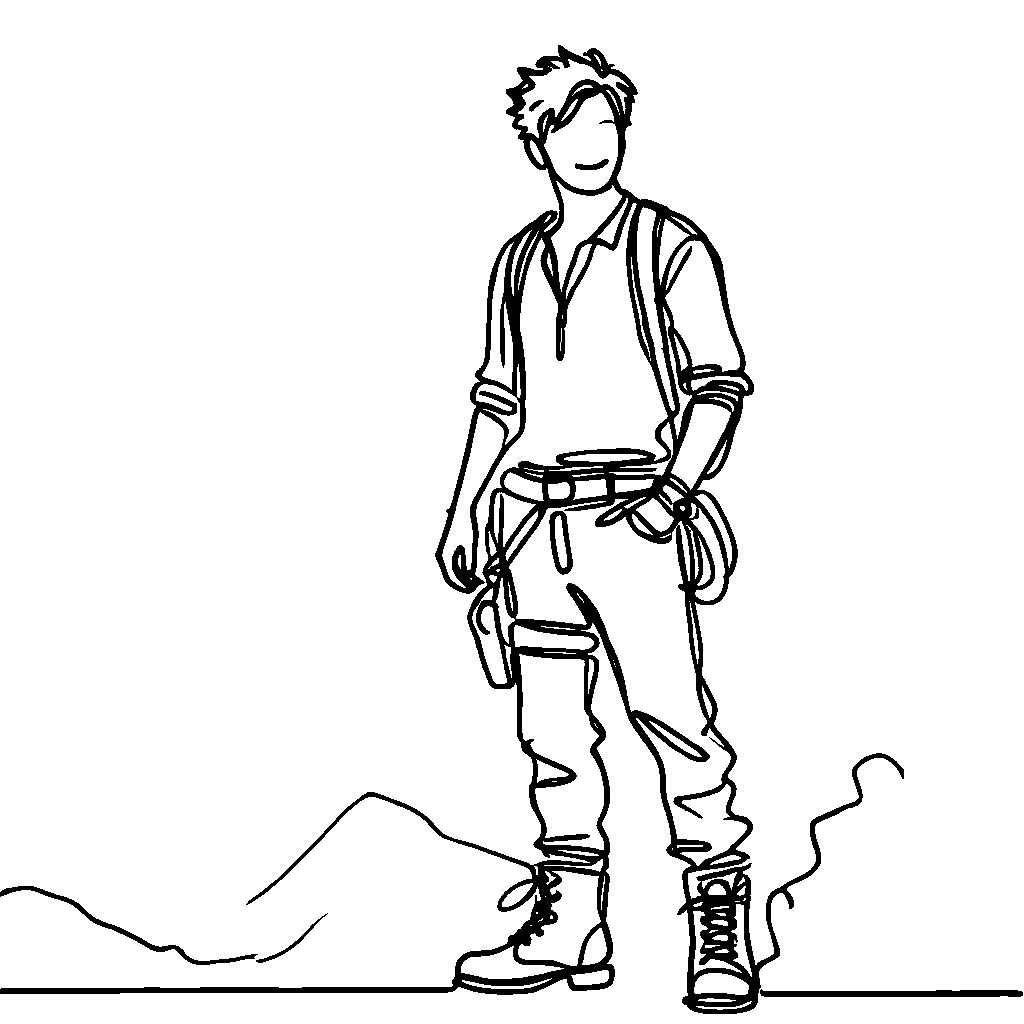
\includegraphics[width=\linewidth]{../presentations/images/lecture_8/urtreasurehunter.jpg}
            \end{column}
    
            \begin{column}{0.7\textwidth}
                Imagine you're part of a treasure hunt...
            \end{column}
        \end{columns}

        \pause

        \begin{columns}
            \begin{column}{0.7\textwidth}
                ...and you've found a hidden treasure chest...
            \end{column}

            \begin{column}{0.2\textwidth}
                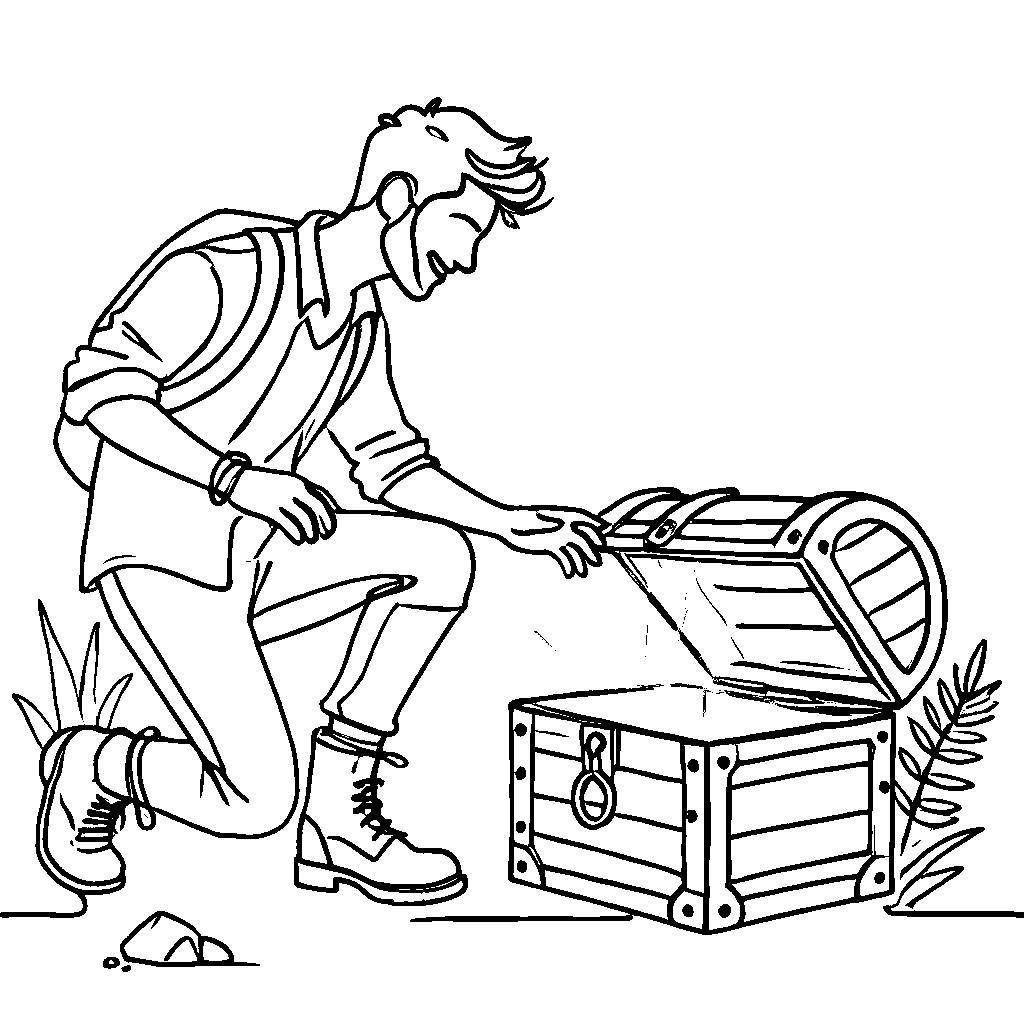
\includegraphics[width=\linewidth]{../presentations/images/lecture_8/uvefoundtreasure.jpg}
            \end{column}
        \end{columns}

        \pause

        \begin{columns}
            \begin{column}{0.2\textwidth}
                
\includegraphics[width=\linewidth]{../presentations/images/lecture_8/howtomakeaproof.jpg}
            \end{column}

            \begin{column}{0.7\textwidth}
                ...but how to prove that without revealing the chest location?
            \end{column}
        \end{columns}
    \end{frame}

    \begin{frame}{Still didn't get who is Snark...}
        \begin{columns}
            \begin{column}{0.65\textwidth}
                \textbf{The Problem}: you have found a hidden treasure chest, and you want to 
                prove to the organizer that you know its location without actually revealing that.
            \end{column}

            \begin{column}{0.3\textwidth}
                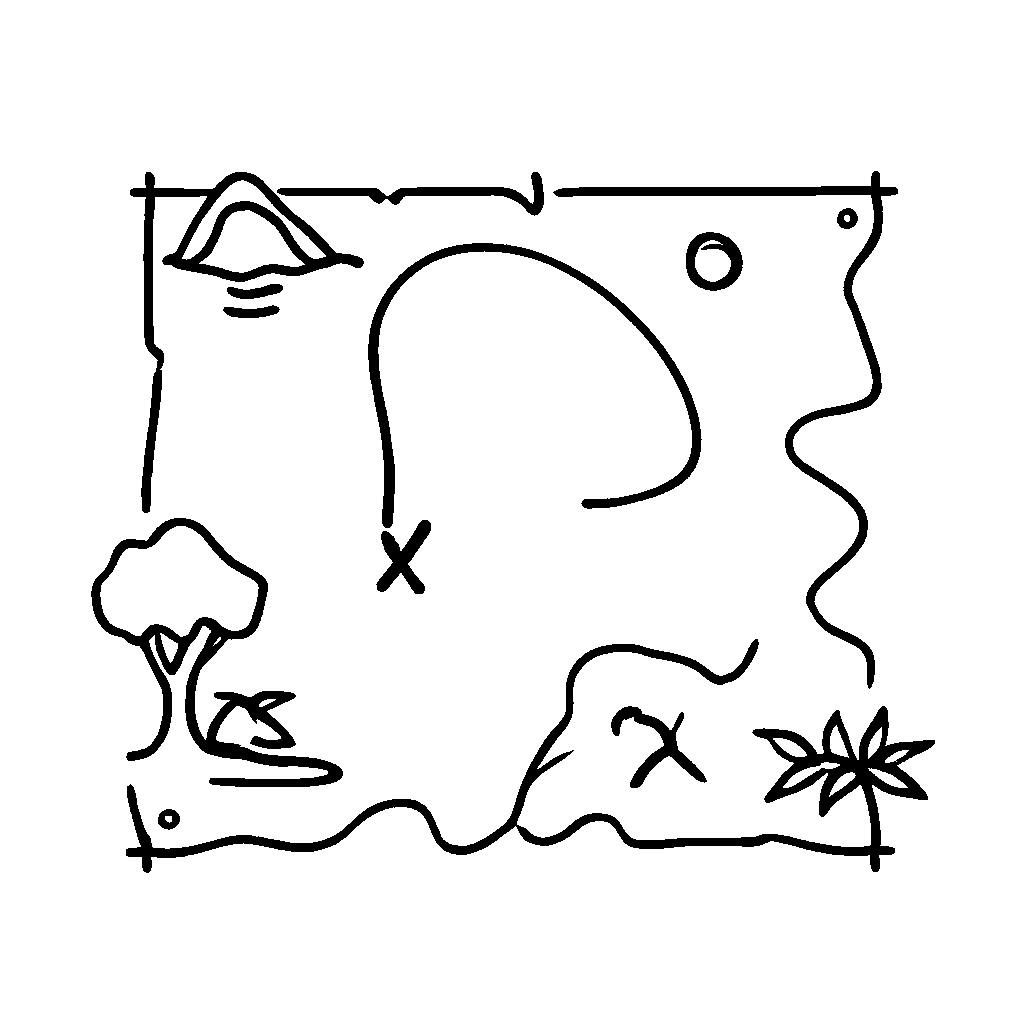
\includegraphics[width=\textwidth]{../presentations/images/lecture_8/treasurelocation.jpg}
            \end{column}
        \end{columns}

        \pause

        We can retrieve some information from that:

        \begin{alertblock}{Question \#81673}
            What is a secret data? Who is a prover and who is a verifier?            
        \end{alertblock}

        \pause

        \vspace{0.1cm}
        \textbf{The Secret Data}: the exact treasure location.

        \vspace{0.1cm}
        \textbf{The Prover}: you.

        \vspace{0.1cm}
        \textbf{The Verifier}: the treasure hunt organizer.
    \end{frame}

    \begin{frame}{Ohh... Got it!}
        Here is how we can apply the zk-SNARK to our problem:

        \begin{itemize}
            \item Argument of Knowledge: You need to create a proof that demonstrates you know the
            chest is. \pause
            \item Succinct: The proof you provide is very small and concise. It doesn't matter how
            large the treasure map is or how many steps it took you to find the chest. \pause
            \item Non-interactive: You don't need to have a back-and-forth conversation with the 
            organizer to create this proof. \pause
            \item Zero-Knowledge: The proof doesn't reveal any information about the actual 
            location of the treasure chest.
        \end{itemize}

        \pause

        \begin{columns}
            \begin{column}{0.3\textwidth}
                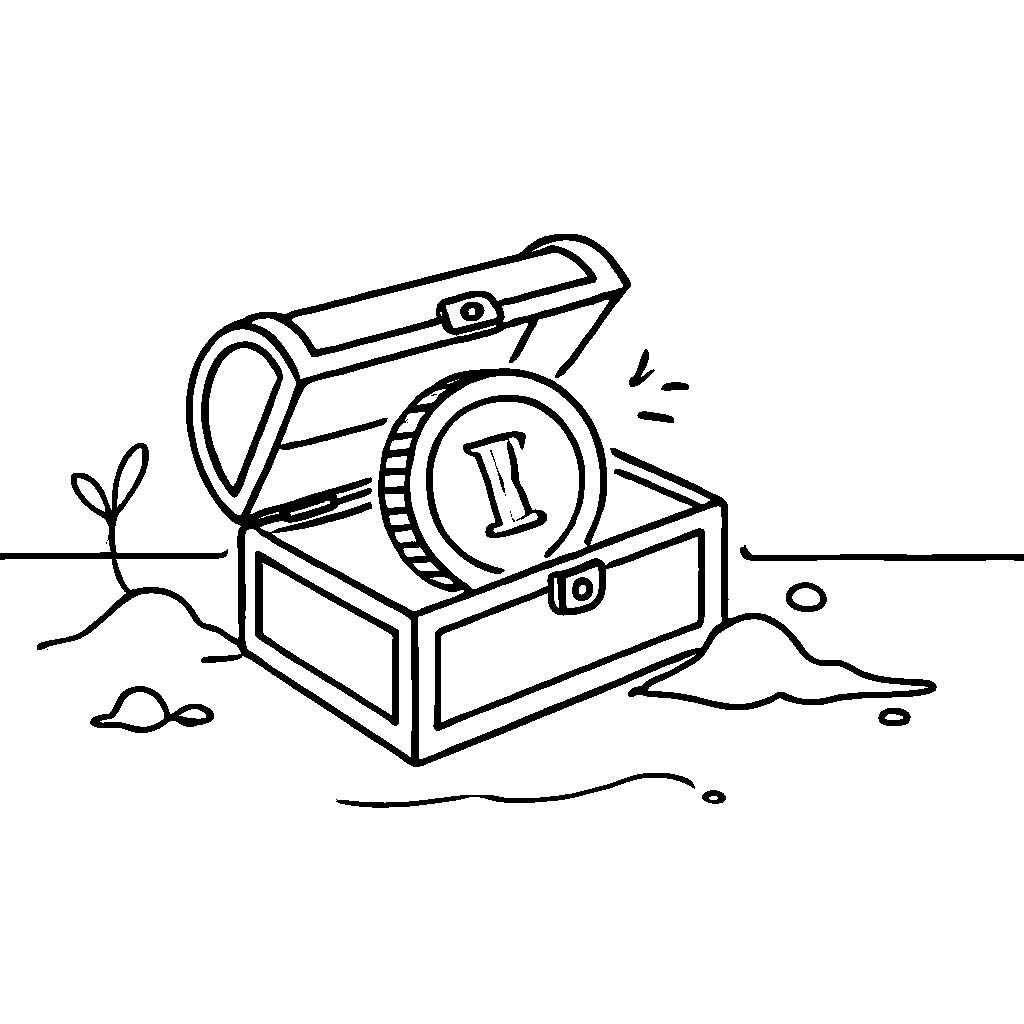
\includegraphics[width=\textwidth]{../presentations/images/lecture_8/treasure.jpg}
            \end{column}

            \begin{column}{0.65\textwidth}
                Well... The golden coin where the pirates' sign is engraved is our zk-SNARK proof!
            \end{column}
        \end{columns}
    \end{frame}

    \begin{frame}
        But the problems that we usually want to solve are in a slightly different format.

        \pause

        \vspace{0.2cm}
        When we need to prove that some element is in a merkle tree, we can't come
        to a verifier and give them a "coin"...

        \center
        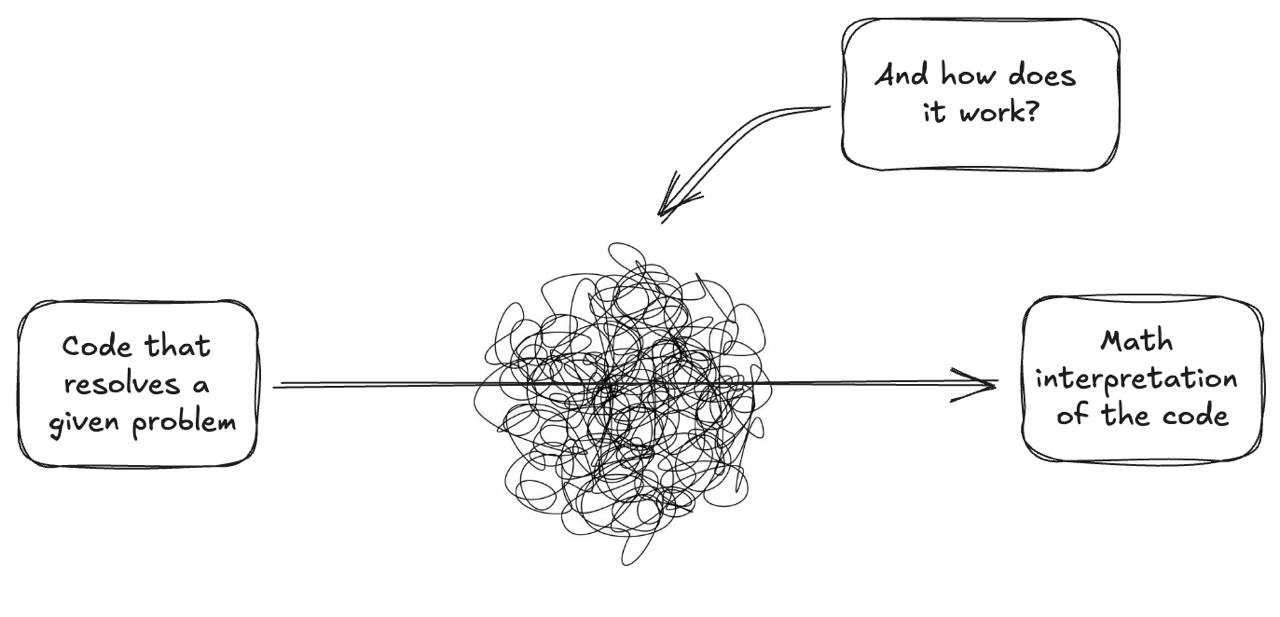
\includegraphics[width=10cm]{../presentations/images/lecture_8/exactcodetomathflow.jpg}
    \end{frame}

    \section{Boolean Circuits}

    \begin{frame}{The First Question To Resolve}
        The cryptographic tools we have learned in the previous lectures operate with numbers or
        certain primitives above them. 
        
        \begin{alertblock}{Question?}
            How do we convert a program into a mathematical language?
        \end{alertblock}

        \vspace{1cm}
        Do not forget about succintness!
    \end{frame}

    \begin{frame}{Boolean Circuits}
        We can do that in a way like the computer does it - boolean circuits.

        % --- Writing diagrams ---
        % Define circle styles and colors
        \colorlet{circle edge}{gray!50!black}
        \colorlet{circle area}{gray!20}
        \colorlet{gate1 edge}{green!50!black}
        \colorlet{gate1 area}{green!20}
        \colorlet{gate2 edge}{orange!50!black}
        \colorlet{gate2 area}{orange!20}
        \colorlet{gate3 edge}{blue!50!black}
        \colorlet{gate3 area}{blue!20}

        \tikzset{
            var/.style={circle, draw=circle edge, fill=circle area, very thick, minimum size=0.7cm, text centered},
            gate1/.style={circle, draw=gate1 edge, fill=gate1 area, ultra thick, minimum size=1cm, text centered},
            gate2/.style={circle, draw=gate2 edge, fill=gate2 area, ultra thick, minimum size=1cm, text centered},
            gate3/.style={circle, draw=gate3 edge, fill=gate3 area, ultra thick, minimum size=1cm, text centered},
            arrow/.style={-latex, ultra thick}
        }

        \begin{figure}[h!]
            \centering
            
            \begin{minipage}{0.54\textwidth}
                \centering
                % Boolean AND and OR gates
                \begin{tabular}{cc}
                    \begin{tikzpicture}
                        % Nodes
                        \node[var] (a) at (0, -1.5) {$a$};
                        \node[var] (b) at (2, -1.5) {$b$};
                        \node[gate1] (and) at (1, 0) {\texttt{AND}};
                        \node[var] (c) at (1, 1.75) {$c$};
        
                        % Arrows
                        \draw[arrow,gray] (a) -- (and);
                        \draw[arrow,gray] (b) -- (and);
                        \draw[arrow,gray!50!black] (and) -- (c);
                    \end{tikzpicture}
                    &
                    \begin{tikzpicture}
                        % Nodes
                        \node[var] (a) at (0, -1.5) {$a$};
                        \node[var] (b) at (2, -1.5) {$b$};
                        \node[gate2] (or) at (1, 0) {\texttt{OR}};
                        \node[var] (c) at (1, 1.75) {$c$};
        
                        % Arrows
                        \draw[arrow,gray] (a) -- (or);
                        \draw[arrow,gray] (b) -- (or);
                        \draw[arrow,gray!50!black] (or) -- (c);
                    \end{tikzpicture}
                \end{tabular}
                \centering
                \caption{Boolean \texttt{AND} and \texttt{OR} Gates}
            \end{minipage}
            \hspace{0.05\textwidth} % Space between figures
            \pause
            \begin{minipage}{0.36\textwidth}
                \centering
                \begin{tabular}{|c|c|c|}
                    \hline
                    \textbf{A} & \textbf{B} & \textbf{A AND B} \\
                    \hline
                    0 & 0 & 0 \\
                    \hline
                    0 & 1 & 0 \\
                    \hline
                    1 & 0 & 0 \\
                    \hline
                    1 & 1 & 1 \\
                    \hline
                \end{tabular}
                \caption{\texttt{AND} Gate Truth Table}
            \end{minipage}
        \end{figure}

        \begin{block}{Note}
        With any of \{\texttt{AND}, \texttt{NOT}\} or \{\texttt{OR}, \texttt{NOT}\} gates sets one can
        build any possible logical circuit, they are called \textbf{functionally complete} sets.
        \end{block}
    \end{frame}

    \begin{frame}{Boolean Circuit Example}
        % --- Writing diagrams ---
        % Define circle styles and colors
        \colorlet{circle edge}{gray!50!black}
        \colorlet{circle area}{gray!20}
        \colorlet{gate1 edge}{green!50!black}
        \colorlet{gate1 area}{green!20}
        \colorlet{gate2 edge}{orange!50!black}
        \colorlet{gate2 area}{orange!20}
        \colorlet{gate3 edge}{blue!50!black}
        \colorlet{gate3 area}{blue!20}

        \tikzset{
            var/.style={circle, draw=circle edge, fill=circle area, very thick, minimum size=0.7cm, text centered},
            gate1/.style={circle, draw=gate1 edge, fill=gate1 area, ultra thick, minimum size=1cm, text centered},
            gate2/.style={circle, draw=gate2 edge, fill=gate2 area, ultra thick, minimum size=1cm, text centered},
            gate3/.style={circle, draw=gate3 edge, fill=gate3 area, ultra thick, minimum size=1cm, text centered},
            arrow/.style={-latex, ultra thick}
        }

        \begin{figure}[h!]
            \centering
            \begin{tikzpicture}
                % Nodes
                \node[var] (a) at (0, -1.5) {$a$};
                \node[var] (b) at (2, -1.5) {$b$};
                \node[var] (c) at (4, -1.5) {$c$};
                \node[gate1] (and) at (1, 0) {\texttt{AND}};
                \node[gate2] (or) at (3, 1.5) {\texttt{OR}};
                \node[var] (d) at (5, 1.5) {$d$};
        
                % Arrows
                \draw[arrow,gray] (a) -- (and);
                \draw[arrow,gray] (b) -- (and);
                \draw[arrow,gray] (c) -- (or);
                \draw[arrow,gray] (and) -- (or);
                \draw[arrow,gray!50!black] (or) -- (d);
            \end{tikzpicture}
            \vspace{-5pt}
            \caption{Example of a circuit evaluating $d = (a \;\texttt{AND}\; b) \,\texttt{OR}\; c$.}
        \end{figure}\pause
        \vspace{-5pt}
        Boolean circuits receive an input vector of {0, 1} and resolve to true (1) or false (0); 
        basically, they determine if the input values satisfy the statement.\\
        \vspace{5pt}
        The above circuit can be satisfied with the next values:
        \vspace{-5pt}
        \begin{equation*}
            a = 1, \quad b = 1, \quad c = 0
        \end{equation*}
    \end{frame}

    \begin{frame}{SHA-256 Boolean circuit}
        \begin{figure}[h!]
            \centering
            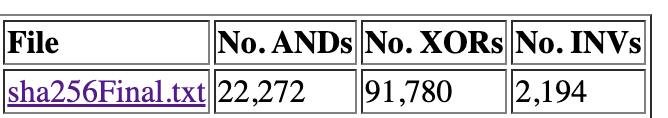
\includegraphics[width=8cm]{../presentations/images/lecture_8/sha256booleancircuit.jpg}
            \vspace{-10pt}  % Reduce the vertical space between the image and the caption
            \caption{Stats of a SHA256 boolean circuit implementation.}
        \end{figure}
        More than $100000$ gates. Impressive, doesn't it? \\
        \vspace{5pt }
        But it also shows how inconvenient the boolean circuits are. 
    \end{frame}

    \section{Arithmetic Circuits}

    \begin{frame}{Arithmetic Circuits}
        Similar to Boolean Circuits, the \textbf{Arithmetic circuits} consist of gates and
        wires. 
        \begin{itemize}
            \item Wires: elements of some finite field $\mathbb{F}$.
            \item Gates: addition ($\oplus$) and multiplication ($\odot$) corresponding to the field.
        \end{itemize} 

        % --- Writing diagrams ---
        % Define circle styles and colors
        \colorlet{circle edge}{gray!50!black}
        \colorlet{circle area}{gray!20}
        \colorlet{gate1 edge}{green!50!black}
        \colorlet{gate1 area}{green!20}
        \colorlet{gate2 edge}{orange!50!black}
        \colorlet{gate2 area}{orange!20}
        \colorlet{gate3 edge}{blue!50!black}
        \colorlet{gate3 area}{blue!20}

        \tikzset{
            var/.style={circle, draw=circle edge, fill=circle area, very thick, minimum size=0.7cm, text centered},
            gate1/.style={circle, draw=gate1 edge, fill=gate1 area, ultra thick, minimum size=1cm, text centered},
            gate2/.style={circle, draw=gate2 edge, fill=gate2 area, ultra thick, minimum size=1cm, text centered},
            gate3/.style={circle, draw=gate3 edge, fill=gate3 area, ultra thick, minimum size=1cm, text centered},
            arrow/.style={-latex, ultra thick}
        }

        \begin{figure}[h!]
            \centering
            % Addition and Multiplication gates
            \begin{tabular}{cc}
                \begin{tikzpicture}
                    % Nodes
                    \node[var] (a) at (0, -1.5) {$a$};
                    \node[var] (b) at (2, -1.5) {$b$};
                    \node[gate1] (add) at (1, 0) {$+$};
                    \node[var] (c) at (1, 1.75) {$c$};

                    % Arrows
                    \draw[arrow,gray] (a) -- (add);
                    \draw[arrow,gray] (b) -- (add);
                    \draw[arrow,gray!50!black] (add) -- (c);
                \end{tikzpicture}
                &
                \begin{tikzpicture}
                    % Nodes
                    \node[var] (a) at (0, -1.5) {$a$};
                    \node[var] (b) at (2, -1.5) {$b$};
                    \node[gate2] (mul) at (1, 0) {$\times$};
                    \node[var] (c) at (1, 1.75) {$c$};

                    % Arrows
                    \draw[arrow,gray] (a) -- (mul);
                    \draw[arrow,gray] (b) -- (mul);
                    \draw[arrow,gray!50!black] (mul) -- (c);
                \end{tikzpicture}
            \end{tabular}
            \caption{Addition and Multiplication Gates}
        \end{figure}
    \end{frame}
 
    \begin{frame}[fragile]{Arithmetic Circuits Example I}
        \begin{example}
            \begin{lstlisting}[language=Python, numbers=none, autogobble=true, xleftmargin=10pt]
                def multiply(a: F, b: F) -> F:
                    return a * b
            \end{lstlisting}
            \pause
            This can be represented as a circuit with only one (multiplication) gate:
            \begin{equation*}
                r = a \times b
            \end{equation*}    
            \pause
            The witness vector (essentially, our solution vector) is $\mathbf{w} = (r, a, b)$, for
            example: $(6, 2, 3)$. \\
            \vspace{5pt}
            We assume that the $a$ and $b$ are input values.
        \end{example}

        \pause

        \begin{block}{Note}
            We can think of the ``=`` in the gate as an assertion.
        \end{block}
    \end{frame}

    \begin{frame}[fragile]{Arithmetic Circuits Example II}
        \begin{example}
            Now, suppose we want to implement the evaluation of the polynomial
            $Q(x_1,x_2) = x_1^3 + x_2^2 \in \mathbb{F}[x_1,x_2]$ using arithmetic circuits.
            \begin{lstlisting}[language=Python, numbers=none, autogobble=true, xleftmargin=10pt]
                def evaluate(x1: F, x2: F) -> F:
                    return x1**3 + x2**2
            \end{lstlisting}
            Looks easy, right? But the circuit is now much less trivial.
            \vspace{-8pt}
            \begin{equation*}
                \begin{array}{c c c}
                    \begin{aligned}
                        x_1^2 &= x_1 \times x_1 \\
                        x_1^3 &= x_1^2 \times x_1 \\
                        x_2^2 &= x_2 \times x_2 \\
                        Q &= x_1^3 + x_2^2 
                    \end{aligned}
                    & \text{or} &
                    \begin{aligned}
                        r_1 &= x_1 \times x_1 \\
                        r_2 &= r_1 \times x_1 \\
                        r_3 &= x_2 \times x_2 \\
                        Q &= r_2 + r_3 
                    \end{aligned}
                \end{array}
            \end{equation*}
        \end{example}
    \end{frame}

    \begin{frame}[fragile]{Arithmetic Circuits Example II}
        % Define circle styles and colors
        \colorlet{circle edge}{gray!50!black}
        \colorlet{circle area}{gray!20}
        \colorlet{gate1 edge}{green!50!black}
        \colorlet{gate1 area}{green!20}
        \colorlet{gate2 edge}{orange!50!black}
        \colorlet{gate2 area}{orange!20}
        \colorlet{gate3 edge}{blue!50!black}
        \colorlet{gate3 area}{blue!20}

        \tikzset{
            var/.style={circle, draw=circle edge, fill=circle area, very thick, minimum size=0.7cm, text centered},
            gate1/.style={circle, draw=gate1 edge, fill=gate1 area, ultra thick, minimum size=1cm, text centered},
            gate2/.style={circle, draw=gate2 edge, fill=gate2 area, ultra thick, minimum size=1cm, text centered},
            gate3/.style={circle, draw=gate3 edge, fill=gate3 area, ultra thick, minimum size=1cm, text centered},
            arrow/.style={-latex, ultra thick}
        }
        
        \begin{figure}[h!]
            \centering
            \begin{tikzpicture}
                % Nodes
                \node[var] (x1) at (0, 1) {$x_1$};
                \node[gate2] (x1_x1) at (2, 1) {$\times$};
                \node[gate2] (x1_x1_x1) at (4, 1) {$\times$};
        
                \node[var] (x2) at (0, -1) {$x_2$};
                \node[gate2] (x2_x2) at (2, -1) {$\times$};
        
                \node[gate1] (plus) at (5.0, -0.5) {$+$};
        
                % x1**3
                \draw[arrow,gray] (x1) to [bend left=45] (x1_x1);
                \draw[arrow,gray] (x1) to [bend right=15] (x1_x1);
                \draw[arrow,gray] (x1_x1) -- (x1_x1_x1);
                \draw[arrow,gray] (x1) to [bend right=45] (x1_x1_x1);
        
                % x2**2
                \draw[arrow,gray] (x2) to [bend left=30] (x2_x2);
                \draw[arrow,gray] (x2) to [bend right=30] (x2_x2);
        
                % Summation
                \draw[arrow,gray] (x1_x1_x1) -- (plus);
                \draw[arrow,gray] (x2_x2) -- (plus);
        
                % Result
                \node[var] (q) at (7.0, -0.5) {$Q$};
                \draw[arrow,gray!50!black] (plus) -- (q);
            \end{tikzpicture}
            \caption{Example of a circuit evaluating $x_1^3 + x_2^2$.}
        \end{figure}
    \end{frame}

    \begin{frame}[fragile]{Arithmetic Circuits Example III}
        \begin{example}
            Well, it is quite clear how to represent any polynomial-like expressions. But how can we
            translate \texttt{if} statements?
            \begin{lstlisting}[language=Python, numbers=none, autogobble=true, xleftmargin=8pt]
                def example(a: bool, b: F, c: F) -> F:
                    if a:
                        return b * c 
                    else:
                        return b + c
            \end{lstlisting}
            \pause
            We can transform such a function into the next expression:
            \vspace{-8pt}
            \begin{equation*}
                r = a \times (b \times c) + (1 - a) \times (b + c)    
                \vspace{-8pt}
            \end{equation*}
            \pause
            Corresponding equations for the circuit are:
            \vspace{-8pt}
            \begin{equation*}
                \begin{aligned}
                    r_1 &= b \times c, \quad &r_3 &= 1 - a, \quad &r_5 &= r_3 \times r_2 \\
                    r_2 &= b + c, \quad &r_4 &= a \times r_1, \quad &r &= r_4 + r_5
                \end{aligned}
            \end{equation*}
        \end{example}
    \end{frame}

    \begin{frame}[fragile]{Arithmetic Circuits Example III}
        % Define circle styles and colors
        \colorlet{circle edge}{gray!50!black}
        \colorlet{circle area}{gray!20}
        \colorlet{gate1 edge}{green!50!black}
        \colorlet{gate1 area}{green!20}
        \colorlet{gate2 edge}{orange!50!black}
        \colorlet{gate2 area}{orange!20}
        \colorlet{gate3 edge}{blue!50!black}
        \colorlet{gate3 area}{blue!20}

        \tikzset{
            var/.style={circle, draw=circle edge, fill=circle area, very thick, minimum size=0.7cm, text centered},
            gate1/.style={circle, draw=gate1 edge, fill=gate1 area, ultra thick, minimum size=1cm, text centered},
            gate2/.style={circle, draw=gate2 edge, fill=gate2 area, ultra thick, minimum size=1cm, text centered},
            gate3/.style={circle, draw=gate3 edge, fill=gate3 area, ultra thick, minimum size=1cm, text centered},
            arrow/.style={-latex, ultra thick}
        }

        \begin{figure}[h!]
            \centering
            \begin{tikzpicture}
                % Nodes
                \node[var] (c) at (0.5, -3) {$c$};
                \node[var] (b) at (0.5, -1.5) {$b$};
                \node[var] (a) at (0.5, 0) {$a$};
                \node[var] (one) at (0.5, 1.5) {$1$};
        
                % b+c and b*c gates
                \node[gate1] (b_plus_c) at (3, -1.5) {$+$};
                \node[gate2] (b_times_c) at (3, -3.0) {$\times$};
        
                \node[gate3] (one_minus_a) at (3, 0.75) {$-$};
        
                % a*b*c and (1-a)(b+c) gates
                \node[gate2] (a_times_b_times_c) at (6, -2.0) {$\times$};
                \node[gate2] (one_minus_a_times_b_plus_c) at (6, -0.5) {$\times$};
        
                % a*b*c + (1-a)(b+c) gate
                \node[gate1] (r) at (9, -1.25) {$+$};
        
                % Result node
                \node[var] (result) at (11.5, -1.25) {$r$};
        
                % b+c and b*c arrows
                \draw[arrow,gray] (b) to (b_plus_c);
                \draw[arrow,gray] (b) to (b_times_c);
                \draw[arrow,gray] (c) to (b_plus_c);
                \draw[arrow,gray] (c) to (b_times_c);
        
                % 1 - c arrow
                \draw[arrow,gray] (one) to (one_minus_a);
                \draw[arrow,gray] (a) to (one_minus_a);
        
                % a*b*c and (1-a)(b+c) arrows
                \draw[arrow,gray] (a) to [bend left=20] (a_times_b_times_c);
                \draw[arrow,gray] (b_times_c) to node[midway, above] {$r_1$} (a_times_b_times_c);
                \draw[arrow,gray] (one_minus_a) to node[midway, above] {$r_3$} (one_minus_a_times_b_plus_c);
                \draw[arrow,gray] (b_plus_c) to node[midway, above] {$r_2$} (one_minus_a_times_b_plus_c);
        
                % a*b*c + (1-a)(b+c) arrows
                \draw[arrow,gray] (a_times_b_times_c) to [bend right=20] node[midway, above] {$r_4$} (r);
                \draw[arrow,gray] (one_minus_a_times_b_plus_c) to [bend left=20] node[midway, above] {$r_5$} (r);
        
                % Result arrow
                \draw[arrow,gray!50!black] (r) to (result);
        
            \end{tikzpicture}
            \caption{Example of a circuit evaluating the \texttt{if} statement logic.}
            \label{fig:multivariate-polynomial-circuit}
        \end{figure}
    \end{frame}

    \begin{frame}{Circuit Satisfability Problem}
        \begin{definition}
            Arithmetic circuit $\mathtt{C}: \mathbb{F}^N \to \mathbb{F}$ over a finite field 
            $\mathbb{F}$ is a directed acyclic graph where internal nodes are labeled via 
            \texttt{+}, \texttt{-}, and $\times$, and inputs are labeled $1,x_1,x_2,\dots,x_n$. 
            By $|\mathtt{C}|$ we denote the number of gates in the circuit.
        \end{definition}
        \pause
        \begin{definition}
            The \textbf{Circuit Satisfiability Problem} is defined as follows: given an arithmetic 
            circuit $\mathtt{C}$ and a public input $x \in \mathbb{F}^n$, determine if there exists 
            a private input $w \in \mathbb{F}^m$ such that $\mathtt{C}(x,w) = 0$. More formally, the
            problem is determined by relation $\mathcal{R}_{\texttt{C}}$ and corresponding language
            $\mathcal{L}_{\texttt{C}}$ as follows:
            \begin{align*}
                \mathcal{R}_{\texttt{C}} &= \{(x,w) \in \mathbb{F}^n \times \mathbb{F}^m \; | \; \mathtt{C}(x,w) = 0\},\\ 
                \mathcal{L}_{\texttt{C}} &= \{x \in \mathbb{F}^n \; | \; \exists w \in \mathbb{F}^m: \mathtt{C}(x,w) = 0\}
            \end{align*}
        \end{definition}
    \end{frame}

    \section{Linear Algebruh Preliminaries}

    \begin{frame}{Vector Space}
        \begin{definition}
            A \textbf{vector space} $V$ over the field $\mathbb{F}$ is an abelian group for addition
            ``$+$`` together with a scalar multiplication operation ``$\cdot$`` from $\mathbb{F} \times V$
            to $V$, sending $(\lambda,x) \mapsto \lambda x$ and such that for any 
            $\mathbf{v},\mathbf{u} \in V$ and $\lambda,\mu \in \mathbb{F}$ we have:
            \begin{itemize}
                \item $\lambda(\mathbf{u}+\mathbf{v}) = \lambda \mathbf{u} + \lambda \mathbf{v}$
                \item $(\lambda + \mu)\mathbf{v} = \lambda \mathbf{v} + \mu \mathbf{v}$
                \item $(\lambda \mu)\mathbf{v} = \lambda(\mu \mathbf{v})$
                \item $1\mathbf{v} = \mathbf{v}$
            \end{itemize}

            Any element $\mathbf{v} \in V$ is called a \textbf{vector}, and any element
            $\lambda \in \mathbb{F}$ is called a \textbf{scalar}. We also mark vector elements in 
            boldface.
        \end{definition}
    \end{frame}

    \begin{frame}{Matrix}
        The matrix is a rectangular array of numbers, symbols, or expressions, arranged in rows and 
        columns. For example, the matrix $A$ with $m$ rows and $n$ columns, consisting of elements 
        from the finite field $\mathbb{F}$ is denoted as $A \in \mathbb{F}^{m \times n}$. 

        \begin{definition}
            Let $A,B$ be two matrices over the field $\mathbb{F}$. The following operations are defined:
            \begin{itemize}
                \item \textbf{Matrix addition/subtraction}: $A \pm B = \{a_{i,j} \pm b_{i,j}\}_{i,j=1}^{m \times n}$. The matrices $A$ and $B$ must have the same size $m \times n$.
                \item \textbf{Scalar multiplication}: $\lambda A = \{\lambda a_{i,j}\}_{1\leq i,j \leq n}$ for any $\lambda \in \mathbb{F}$.
                \item \textbf{Matrix multiplication}: $C = AB$ is a matrix $C \in \mathbb{F}^{m \times p}$ with elements $c_{i,j} = \sum_{\ell=1}^{n} a_{i,\ell}b_{\ell,j}$. The number of columns in $A$ must be equal to the number of rows in $B$, that is $A \in \mathbb{F}^{m \times n}$ and $B \in \mathbb{F}^{n \times p}$.
            \end{itemize}
        \end{definition}
    \end{frame}

    \begin{frame}{Matrix Multiplication}
        \begin{example}
            Consider 
            \begin{equation*}
                A = \begin{bmatrix}
                    1 & 1 & 2 \\
                    2 & 2 & 1
                \end{bmatrix} \in \mathbb{R}^{2 \times 3}, \quad B = \begin{bmatrix}
                    2 & 1 \\
                    1 & 3 \\
                    1 & 1
                \end{bmatrix} \in \mathbb{R}^{3 \times 2}
            \end{equation*}
        
            We cannot add $A$ and $B$ since they have different sizes. However, we can multiply them:
            \begin{equation*}
                AB = \begin{bmatrix}
                    5 & 6 \\ 7 & 9
                \end{bmatrix}, \quad BA = \begin{bmatrix}
                    4 & 4 & 5 \\
                    7 & 7 & 5 \\
                    3 & 3 & 3
                \end{bmatrix}
            \end{equation*}
        
            To see why, for example, the upper left element of $AB$ is $5$, we can calculate it as 
            $\sum_{\ell=1}^3 a_{1,\ell}b_{\ell,1} = 1 \times 2 + 1 \times 1 + 2 \times 1 = 5$.
        \end{example}
    \end{frame}

    \begin{frame}{Vector As A Matrix}
        \begin{block}{Note}
            It just so happens that when working with vectors, we usually assume that they are 
            \textbf{column vectors}. This means that the vector $v = (v_1,v_2,\dots,v_n)$ is 
            represented as a matrix:
            \begin{equation*}
                \mathbf{v} = \begin{bmatrix} v_1 \\ v_2 \\ \vdots \\ v_n \end{bmatrix}
            \end{equation*} 
            This is a common convention in linear algebra, and we will use it in the following 
            sections.
        \end{block}
    \end{frame}

    \begin{frame}{Matrix Transpose}
        \begin{definition}[Transposition]
            Given a matrix $A \in \mathbb{F}^{m \times n}$, the \textbf{transpose} of $A$ is a 
            matrix $A^{\top} \in \mathbb{F}^{n \times m}$ with elements $A^{\top}_{ij} = A_{ji}$.
        \end{definition}
        
        \begin{example}
            \begin{equation*}
                A = \begin{bmatrix} 1 & 2 \\ 3 & 4 \end{bmatrix}, \quad A^{\top} = \begin{bmatrix} 1 & 3 \\ 2 & 4 \end{bmatrix}
            \end{equation*}
            \begin{equation*}
                B = \begin{bmatrix} 1 & 2 & 3 \\ 4 & 5 & 6 \end{bmatrix}, \quad B^{\top} = \begin{bmatrix} 1 & 4 \\ 2 & 5 \\ 3 & 6 \end{bmatrix}
            \end{equation*}
            \begin{equation*}
                \mathbf{v} = \begin{bmatrix} 1 \\ 2 \\ 3 \end{bmatrix}, \quad \mathbf{v}^{\top} = [1,2,3]
            \end{equation*}
        \end{example}
    \end{frame}

    \begin{frame}{Inner Product}
        \begin{definition}
            Consider the vector space $\mathbb{V}$ over the finite field $\mathbb{F}_p$. The 
            \textbf{inner product} is a function 
            $\langle \cdot, \cdot \rangle: \mathbb{V} \times \mathbb{V} \to \mathbb{F}_p$ satisfying 
            the following conditions for all $\mathbf{u},\mathbf{v},\mathbf{w} \in \mathbb{V}$:
            \begin{itemize}
                \item $\langle \mathbf{u} + \mathbf{v}, \mathbf{w} \rangle = \langle \mathbf{u}, \mathbf{w} \rangle + \langle \mathbf{v}, \mathbf{w} \rangle$.
                \item $\langle \mathbf{u}, \mathbf{v} + \mathbf{w} \rangle = \langle \mathbf{u}, \mathbf{v} \rangle + \langle \mathbf{u}, \mathbf{w} \rangle$.
                \item $\langle \mathbf{u}, \mathbf{v} \rangle = 0$ for all $\mathbf{u} \in \mathbb{V}$ iff $\mathbf{v} = \mathbf{0}$.
                \item $\langle \mathbf{u}, \mathbf{v} \rangle = 0$ for all $\mathbf{v} \in \mathbb{V}$ iff $\mathbf{u} = \mathbf{0}$.
            \end{itemize}
        \end{definition}   

        Plenty of functions can be built that satisfy the inner product definition, we'll use the one
        that is usually called \textbf{dot product}.
    \end{frame}

    \begin{frame}{Dot Product}
        \begin{definition}
            Consider the vector space $\mathbb{V}$ over the finite field $\mathbb{F}_p$. The 
            \textbf{dot product} on $\mathbb{V}$ is a function 
            $\langle \cdot, \cdot \rangle: \mathbb{V} \times \mathbb{V} \rightarrow \mathbb{F}$, 
            defined for every $\mathbf{u}, \mathbf{v} \in \mathbb{V}$ as follows:
            \begin{equation*}
                \langle \mathbf{u}, \mathbf{v} \rangle := \mathbf{u}^{\top}\mathbf{v} = \sum_{i=1}^{n} u_i v_i
            \end{equation*}
        \end{definition}

        \pause
        \begin{block}{Note}                 
            The dot product can also be denoted using the dot notation as:
            \vspace{-8pt}
            \begin{equation*}
                \mathbf{u} \cdot \mathbf{v}
                \vspace{-8pt}
            \end{equation*}
            That is why it's called the ``dot`` product.
        \end{block}
    \end{frame}

    \begin{frame}{Dot Product}
        \begin{example}
            Let $\mathbf{u}, \mathbf{v}$ are vectors over the real number $\mathbb{R}$, where
            \begin{equation*}
                \mathbf{u} = (1, 2, 3), \quad \mathbf{v} = (2, 4, 3)
            \end{equation*}
            Then: 
            \begin{equation*}
                \langle \mathbf{u}, \mathbf{v}\rangle = \sum_{i=1}^{3}u_iv_i = 2 \cdot 1 + 2 \cdot 4 + 3 \cdot 3 = 2 + 8 + 9 = 19
            \end{equation*}
        \end{example}
    \end{frame}

    \begin{frame}{Hadamard Product}
        \begin{definition}
            Suppose $A,B \in \mathbb{F}^{m \times n}$. The \textbf{Hadamard product} $A \odot B$ 
            gives a matrix $C$ such that $C_{i,j} = A_{i,j}B_{i,j}$. Essentially, we multiply 
            elements elementwise.
        \end{definition}
        
        \begin{example}
            Consider $A = \begin{bmatrix}
                1 & 1 & 2 \\
                3 & 0 & 3
            \end{bmatrix}, B = \begin{bmatrix}
                3 & 2 & 1 \\ 0 & 2 & 1
            \end{bmatrix}$. Then, the Hadamard product:
            \begin{equation*}
                A \odot B = \begin{bmatrix}
                    1 \cdot 3 & 1 \cdot 2 & 2 \cdot 1 \\
                    3 \cdot 0 & 0 \cdot 2 & 3 \cdot 1
                \end{bmatrix} = \begin{bmatrix}
                    3 & 2 & 2 \\
                    0 & 0 & 3
                \end{bmatrix}
            \end{equation*}
        \end{example}
    \end{frame}

    \begin{frame}{Outer Product}
        \begin{definition}
            Given two vectors $\mathbf{u} \in \mathbb{F}^n$, $\mathbf{v} \in \mathbb{F}^m$ the 
            \textbf{outer product} is a the matrix whose entries are all products of an element in
            the first vector with an element in the second vector:
            \begin{equation*}
                \mathbf{u} \otimes \mathbf{v} := \mathbf{u}\mathbf{v}^{\top} = \begin{bmatrix}
                    u_1 v_1 & u_1 v_2 & \cdots & u_1 v_n \\
                    u_2 v_1 & u_2 v_2 & \cdots & u_2 v_n \\
                    \vdots & \vdots & \ddots & \vdots \\
                    u_m v_1 & u_m v_2 & \cdots & u_m v_n
                \end{bmatrix}
            \end{equation*}
        \end{definition}
    \end{frame}

    \begin{frame}{Outer Product}
        \begin{lemma}[Properties of outer product]
            For any scalar $c \in \mathbb{F}$ and $(\mathbf{u}, \mathbf{v}, \mathbf{w}) \in \mathbb{F}^n \times \mathbb{F}^m \times \mathbb{F}^p$:
            \begin{itemize}
                \item Transpose: $(\mathbf{u} \otimes \mathbf{v}) = (\mathbf{v} \otimes \mathbf{u})^{\textsf{T}}$
                \item Distributivity: $\mathbf{u} \otimes (\mathbf{v} + \mathbf{w}) = \mathbf{u} \otimes \mathbf{v} + \mathbf{u} \otimes \mathbf{w}$
                \item Scalar Multiplication: $c(\mathbf{v} \otimes \mathbf{u}) = (c\mathbf{v}) \otimes \mathbf{u} = \mathbf{v} \otimes (c\mathbf{u})$
                \item Rank: the outer product $\mathbf{u} \otimes \mathbf{v}$ is a rank-1 matrix if $\mathbf{u}$ and $\mathbf{v}$ are non-zero
                vectors
            \end{itemize}
        \end{lemma}
    \end{frame}

    \begin{frame}{Outer Product}
        \begin{example}
            Let $\mathbf{u}, \mathbf{v}$ are vectors over the real number $\mathbb{R}$, where
            \begin{equation*}
                \mathbf{u} = (1, 2, 3), \quad \mathbf{v} = (2, 4, 3)
            \end{equation*}
            Then: 
            \begin{equation*}
                \mathbf{u} \otimes \mathbf{v} = \mathbf{u}\mathbf{v}^{\top} = \begin{bmatrix}
                1 \\ 2 \\ 3
                \end{bmatrix}\begin{bmatrix}
                2 & 4 & 3
                \end{bmatrix} = \begin{bmatrix}
                    1 \cdot 2 & 1 \cdot 4 & 1 \cdot 3 \\
                    2 \cdot 2 & 2 \cdot 4 & 2 \cdot 3 \\
                    3 \cdot 2 & 3 \cdot 4 & 3 \cdot 3
                \end{bmatrix} = \begin{bmatrix}
                    2 & 4 & 3 \\
                    4 & 8 & 6 \\
                    6 & 12 & 9
                \end{bmatrix}
            \end{equation*}

            \pause
            The rows/columns number 2 and 3 in the result matrix can be represented as a linear 
            combination of the first row/column, specifically by multiplying it by 2 and 3, 
            respectively. 
        \end{example}
    \end{frame}

    \section{Rank-1 Constraint System}

    \begin{frame}{Constraint Definition}
        \begin{definition}
            Each \textbf{constraint} in the Rank-1 Constraint System must be in the form:
            \begin{equation*}
                \langle \mathbf{a}, \mathbf{w}\rangle \times \langle \mathbf{b}, \mathbf{w}\rangle = \langle \mathbf{c}, \mathbf{w}\rangle
            \end{equation*}
            Where $\mathbf{w}$ is a vector containing all the \textit{input}, \textit{output}, and 
            \textit{intermediate} variables involved in the computation. The vectors $\mathbf{a}$, 
            $\mathbf{b}$, and $\mathbf{c}$ are vectors of coefficients corresponding to these variables, 
            and they define the relationship between the linear combinations of $\mathbf{w}$ on the 
            left-hand side and the right-hand side of the equation.
        \end{definition}        
    \end{frame}

    \begin{frame}{Constraint Example}
        \begin{example}
            Consider the most basic circuit with one multiplication gate:
            \vspace{-5pt}
            \begin{equation*}
                r = x_1 \times x_2
                \vspace{-5pt}
            \end{equation*}
            Since we have $3$ variables, the constraint is written as:
            \vspace{-5pt}
            \begin{equation*}
                (a_1w_1 + a_2w_2 + a_3w_3)(b_1w_1 + b_2w_2 + b_3w_3) = c_1w_1 + c_2w_2 + c_3w_3
                \vspace{-5pt}
            \end{equation*}
            Coefficients and witness vectors are:
            \vspace{-5pt}
            \begin{equation*}
                \mathbf{w} = (r, x_1, x_2), \quad \mathbf{a} = (0, 1, 0), \quad \mathbf{b} = (0, 0, 1), \quad \mathbf{c} = (1, 0, 0). 
                \vspace{-5pt}
            \end{equation*}
            Therefore, our expression above reduces to:
            \vspace{-5pt}
            \[ (0w_1 + 1w_2 + 0w_3)(0w_1 + 0w_2 + 1w_3) = (1w_1 + 0w_2 + 0w_3) \vspace{-5pt} \]
            \[ w_2 \times w_3 = w_1 \vspace{-5pt} \]
            \[ x_1 \times x_2 = r \]
        \end{example}
    \end{frame}

    \begin{frame}[fragile]{Constraint System Example}
        Now, let us consider a more complex example.
        \begin{lstlisting}[language=Python,numbers=none]
        def r(x1: bool, x2: F, x3: F) -> F:
            return x2 * x3 if x1 else x2 + x3
        \end{lstlisting}
        That can be expressed as:
        \begin{equation*}
            r = x_1 \times (x_2 \times x_3) + (1 - x_1) \times (x_2 + x_3)
        \end{equation*}
        
        \pause
        \begin{alertblock}{}
            We need a boolean restriction for $x_1$:
            \vspace{-8pt}
            \begin{equation*}
                x_1 \times (1 - x_1) = 0
            \end{equation*}
        \end{alertblock}

        \pause
        Thus, the next constraints can be build:
        \vspace{-5pt}
        \begin{align*}
            x_1 \times x_1 &= x_1 \quad \text{(binary check)} \tag{1} \\
            x_2 \times x_3 &= \mathsf{mult} \tag{2} \\
            x_1 \times \mathsf{mult} &= \mathsf{selectMult} \tag{3} \\
            (1 - x_1) \times (x_2 + x_3) &= r - \mathsf{selectMult} \tag{4}
        \end{align*}
    \end{frame}

    \begin{frame}[fragile]{Constraint System Example}
        The witness vector: $\mathbf{w} = (1, r, x_1, x_2, x_3, \mathsf{mult}, \mathsf{selectMult})$.

        \vspace{2pt}
        The coefficients vectors:
        \vspace{-5pt}
        \begin{align*}
            \mathbf{a}_1 &= (0, 0, 1, 0, 0, 0, 0), & \mathbf{b}_1 &= (0, 0, 1, 0, 0, 0, 0), & \mathbf{c}_1 &= (0, 0, 1, 0, 0, 0, 0) \\
            \mathbf{a}_2 &= (0, 0, 0, 1, 0, 0, 0), & \mathbf{b}_2 &= (0, 0, 0, 0, 1, 0, 0), & \mathbf{c}_2 &= (0, 0, 0, 0, 0, 1, 0) \\
            \mathbf{a}_3 &= (0, 0, 1, 0, 0, 0, 0), & \mathbf{b}_3 &= (0, 0, 0, 0, 0, 1, 0), & \mathbf{c}_3 &= (0, 0, 0, 0, 0, 0, 1) \\
            \mathbf{a}_4 &= (1, 0, -1, 0, 0, 0, 0), & \mathbf{b}_4 &= (0, 0, 0, 1, 1, 0, 0), & \mathbf{c}_4 &= (0, 1, 0, 0, 0, 0, -1)
        \end{align*}
        Using the arithmetic in a large finite field $\mathbb{F}_p$, consider the following values:
        \vspace{-10pt}
        \begin{equation*}
            x_1 = 1, \quad x_2 = 3, \quad x_3 = 4
            \vspace{-5pt}
        \end{equation*}
    
        Verifying the constraints:
        \begin{enumerate}
            \item \( x_1 \times x_1 = x_1 \quad (1 \times 1 = 1) \)
            \item \( x_2 \times x_3 = \mathsf{mult} \quad (3 \times 4 = 12) \)
            \item \( x_1 \times \mathsf{mult} = \mathsf{selectMult} \quad (1 \times 12 = 12) \)
            \item \( (1 - x_1) \times (x_2 + x_3) = r - \mathsf{selectMult} \quad (0 \times 7 = 12 - 12) \)
        \end{enumerate}
    \end{frame}

    \begin{frame}{Why Rank-1?}
        \begin{lemma}
            Suppose we have a constraint $\langle \mathbf{a}, \mathbf{w}\rangle \times \langle \mathbf{b}, \mathbf{w}\rangle = \langle \mathbf{c}, \mathbf{w} \rangle$ 
            with coefficient vectors $\mathbf{a}$, $\mathbf{b}$, $\mathbf{c}$ and witness vector 
            $\mathbf{w}$ (all from $\mathbb{F}^n$). Then it can be expressed in the form:
            \vspace{-5pt}
            \begin{equation*}
                 \mathbf{w}^{\top} A \mathbf{w} + \mathbf{c}^{\top} \mathbf{w} = 0
                 \vspace{-5pt}
            \end{equation*}
            Where $A$ is the outer product of vectors $\mathbf{a}$, $\mathbf{b}$, so a \textbf{rank-1} matrix.
        \end{lemma}

        \textbf{Lemma proof.} Consider $\mathbf{a}, \mathbf{b}, \mathbf{c}, \mathbf{w} \in \mathbb{F}^n$.
        \vspace{-5pt}
        \begin{equation*}
            \left(\sum_{i=1}^{n} a_i w_i\right) \times \left(\sum_{j=1}^{n} b_j w_j\right) = \sum_{k=1}^{n} c_k w_k
            \vspace{-5pt}
        \end{equation*}
        Combine the products into a double sum on the left side:
        \vspace{-5pt}
        \begin{equation*}
            \sum_{i=1}^{n} \sum_{j=1}^{n} a_i b_j w_i w_j = \mathbf{w}^{\top} (\mathbf{a} \otimes \mathbf{b}) \mathbf{w} = \mathbf{w}^{\top} A \mathbf{w}
            \vspace{-5pt}
        \end{equation*}
        Thus, the constraint can be written as:
        \vspace{-5pt}
        \begin{equation*}
            \mathbf{w}^{\top} A \mathbf{w} + \mathbf{c}^{\top} \mathbf{w} = 0
            \vspace{-5pt}
        \end{equation*}
    \end{frame}
\end{document}